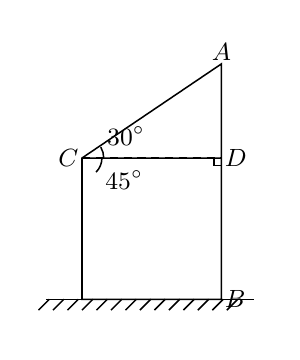
\begin{tikzpicture}[x=.023cm,y=-.023cm,baseline=(current bounding box.center),line width=.55pt,
  every node/.style={font=\small,inner sep=1pt}]
  \path[use as bounding box] (0,0) rectangle (135,168);
  \coordinate (C) at (30,72);
  \coordinate (D) at (107,72);
  \coordinate (A) at (107,20);
  \coordinate (B) at (107,150);
  \draw (30,150)--(30,72)--(A)--(B)--cycle (C)--(D);
  \draw[densely dashed] (C)--(D);
  \draw (C) ++(12,0) arc[start angle=0,end angle=-30,radius=12];
  \draw (C) ++(11,0) arc[start angle=0,end angle=45,radius=11];
  \draw (10,150)--(125,150);
  \foreach \x in {12,20,...,120} {\draw (\x,150)--++(-6,6);}
  \draw (103,72)--(103,76)--(107,76);
  \node[left] at (C) {$C$};
  \node[right] at (D) {$D$};
  \node[above] at (A) {$A$};
  \node[right] at (B) {$B$};
  \node[above right] at (42,67) {$30^\circ$};
  \node[below right] at (41,77) {$45^\circ$};
\end{tikzpicture}
